\chapter{螺管范例,HTS磁体和结论}
\section{引言}
本章包括三个部分。第一部分给出多个螺管磁体范例,各范例均有问题与解答(Q/A)。
第二部分讨论HTS磁体应用及其前景。
最后有一个简明的结论性评论。

这里描述和研究的四个螺管磁体范例的选取,不是因为他们特别重要或唯一---
没有哪个磁体系统是唯一的,不过对某些人而言,每一个磁体都是唯一的。
选取这几个例子,主要还是因为作者对这些磁体的熟悉。
在描述部分之后的Q/A部分,前面七章涉及的设计和运行的若干要点,再次提出。

这里,我们再次强调一下第一章中已经阐述过的我们的基本哲学:
任何问题,需要数值解的,首先应该使用经得起数值解检验的简化模型得到近似估计。
近似估计快速告诉磁体设计者磁体是否在正确的轨道上。
对于任何简单或复杂的磁体,该工作都很重要。
 “创新”磁体的想法通常始于个人。
 为了评估这个想法是否切合实际并且值得与同事进一步深入研究甚至组建设计团队,
 发起人必须首先计算设计和运行关键参数的大概值(第2-8章所述),从简单参数如总安匝数、整体运行电流密度、磁体尺寸和重量、导体总长度,到更复杂的如稳定性和保护、力和低温要求。
 这里的关键词是近似:在磁体项目的后期阶段,设计团队的专家将使用复杂的程序来计算准确的参数值。
 将确切的值留给专家,但要准备好确认他们确实属于独立计算的近似数字范围。
 作者希望在研究了第2-8章后,读者---电磁场、应力、低温、甚至材料领域的专家---
 将能够处理下面提出的四个磁体示例中包含的大多数问题。


\section{螺管磁体示例}
实例中描述和研究的四个螺管磁体是:
1)  由一个大型超导磁体和一个电阻性内插磁体组成的混合磁体;
2) 钢板上的磁体;
3) 一个由螺管磁体产生的磁场悬浮起来的HTS板(盘片);
4) 层叠HTS环组成的“螺管”磁体,HTS环由块材加工或图层导体板构成。 


\subsection{例A:串联混合磁体}
NHMFL建造的中心轴向场35-40 T(取决于室温孔大小,32-50 mm)的高场磁体,由
一个超导磁体和一个5线圈高均匀电阻性(水冷)内插磁体组成。
因为超导磁体和5线圈电阻性内插磁体电气上串联且由同一个DC电源供电,
磁体被称为“串联混合磁体”(series-connected-hybrid, SCH)。
SCH产生的中心场大于NHMFL所有的电阻性磁体的磁场(35 T)或全超导磁体的磁场(21 T)。
图9.1给出了SCH磁体的剖面示意图---
参数值与SCH磁体的最终采纳值略有不同。

SCH还包括一个薄($\alpha\simeq 1$)的超导屏蔽线圈,绕组半径约1 m,图中未画出。
屏蔽线圈的反极性的,用以减小SCH磁体的边缘场。
在Q/A部分,我们将计算超导屏蔽线圈要求的安匝数近似值。
同时,我们还将设计可作为技术备选的钢圆柱壳屏蔽系统。
\begin{figure}[htbp]
	\centering
	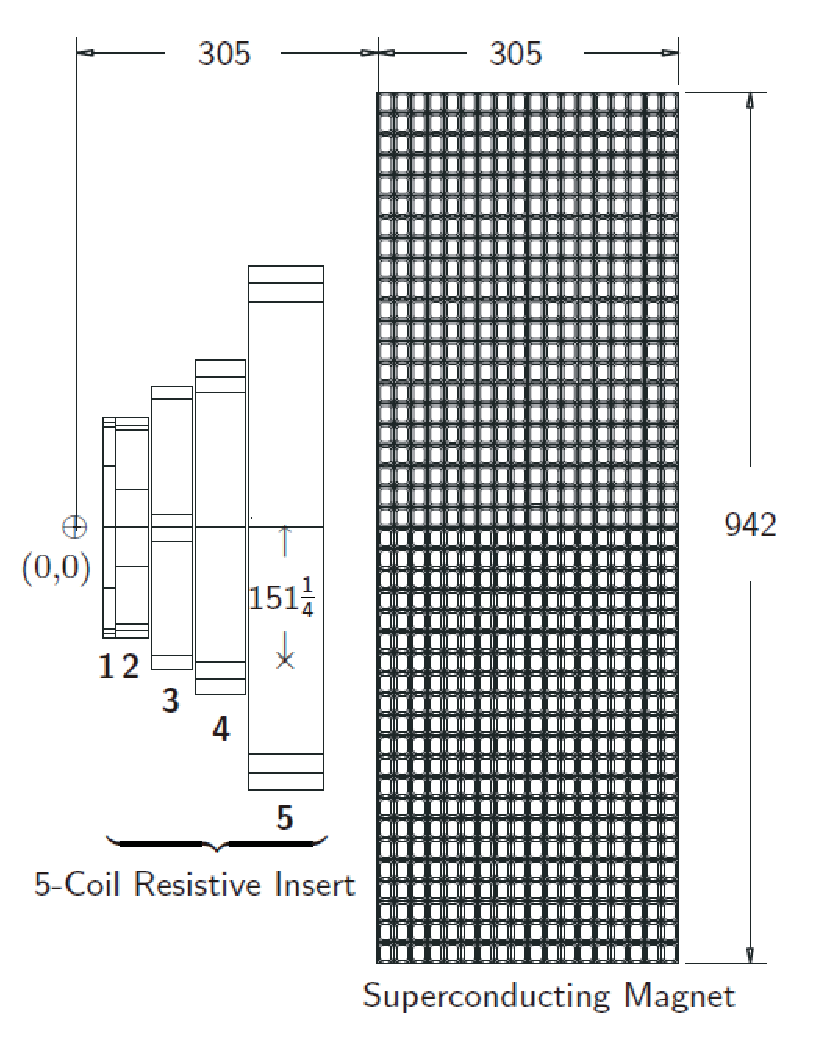
\includegraphics[scale=0.6]{chpt9/figs/fig9.1.eps}
	\caption{NHMFL的SCH磁体的一半结构的剖视图---
		半径约1 m的超导屏蔽线圈未画出。绕组的尺度为近似值,以mm为单位;
	线圈5的$\times$号表示它在故障模式后的磁场中心---将在Q/A部分讨论。}
\end{figure}

\begin{figure}[htbp]
	\centering
	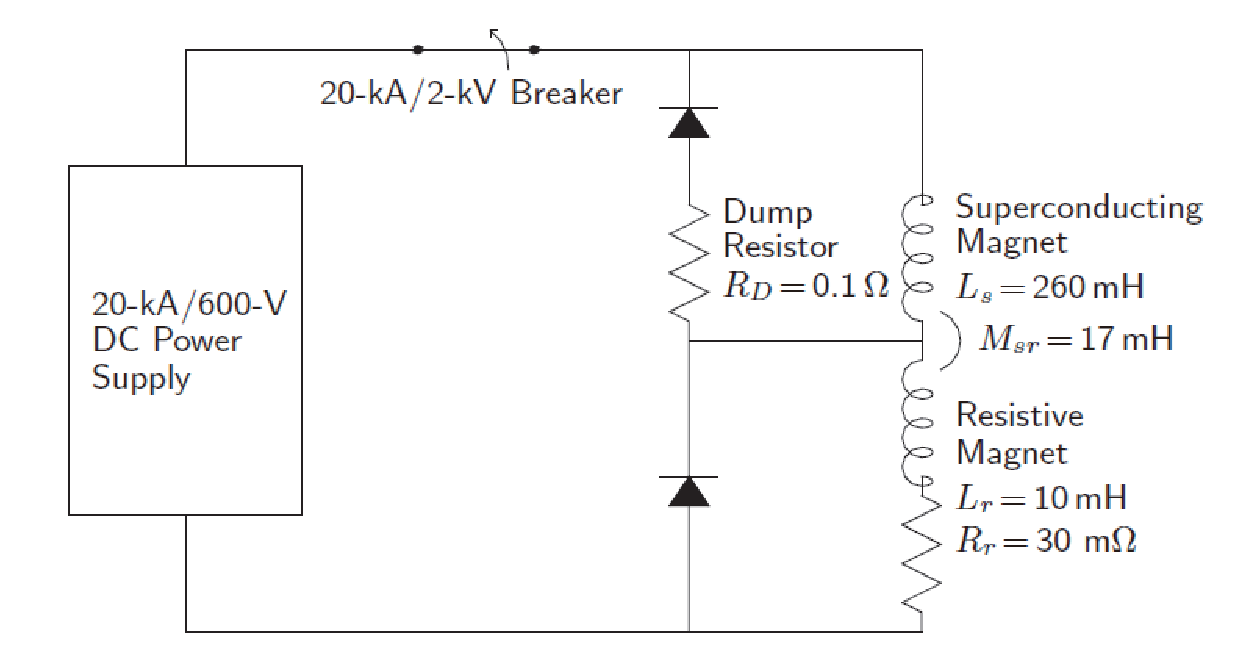
\includegraphics[scale=0.6]{chpt9/figs/fig9.2.eps}
	\caption{SCH磁体的等效电路图。[NHMFL授权使用,2005]}
\end{figure}

图9.2给出了SCH的等效电路图。其中,超导磁体(自感$L_s$=260 mH)与电阻性磁体(自感$L_r$=10 mH,电阻$R_r$=30 m$\Omega$)串联。
磁体由一个20 kA/600 V电源供电。
保护方面,超导磁体用$R_D$=0.1 $\Omega$泄放电阻和二极管串联组作为旁路;
电阻性磁体使用二极管旁路。
(假设两个二极管都是理想的,即正向电阻为零,反向电阻无穷大。)
如图9.2所示,两个磁体间互感$M_{sr}$为17 mH。
在任一磁体异常时,打开20 kA/2 kV断路器。

表9.1列出了超导磁体和该磁体最内层使用的CIC导体的关键参数值。
其中的$A_{sc},A_{\bar{m}},A_{m},A_{cl}$分别是$\mathrm{Nb_3 Sn}$ CIC导体的截面、非基底金属截面、基底金属(铜)截面、4.5 K超临界氦截面。

表9.1.。。。。。。。。。。。。。。

\subsubsection{Q/A A:SCH超导磁体}
\textbf{a) 总体电流密度}\qquad 超导磁体在其运行电流$I_{op}$=20 kA时的总体临界电流密度$\lambda J_{op}$是多少?

\textbf{解:}应用方程3.108a,代入$N$=756和$I=I_{op}$=20 kA,我们得到:
\begin{align*}% page548 第1个
\lambda J_{op}&=\frac{NI}{2b(a_2-a_1)}\\ \tag{3.108a}
&=\frac{756(20\times10^3\ \mathrm{A})}{(942.0\ \mathrm{mm})(610.1\ \mathrm{mm}-305.0\ \mathrm{mm})}=52.6\ \mathrm{A/mm^2}
\end{align*}

\textbf{b) 中心场}\qquad 超导磁体在$I_{op}$=20 kA时,在中心位置产生的磁场(磁感应强度)$B_z(0,0)$是多少?

\textbf{解:}类似的,由表9.1,我们有$\alpha=$1220.2/610.0=2.00;$\beta$=942.0/610.0=1.544。
使用方程3.110,有:
\begin{align*}% page548 第3个
B_{z}(0,0)=\frac{\mu_oNI}{2a_1(\alpha-1)}\ln(\frac{\alpha+\sqrt{\alpha^2+\beta^2}}{1+\sqrt{1+\beta^2}}) \tag{3.110}
\end{align*}

于是,
\begin{align*}% page548 第4个
B_z(0,0)&=\frac{(4\pi\times10^{-7}\ \mathrm{H/m})(756)(20\times10^3\ \mathrm{A})}{(0.610\ \mathrm{m})(2.00-1)}\ln(\frac{2.00+\sqrt{(2.00)^2+(1.544)^2}}{1+\sqrt{1+(1.544)^2}})\\
&=14.52\ \mathrm{T}
\end{align*}

\textbf{c) 中平面径向场}\qquad 超导磁体在中平面($z=0$)的$R=a_2$处产生的磁场的径向分量$B_r(z=0,r=2a_2)$是多少?

\textbf{解:}理想螺管磁体或嵌套线圈磁体产生的磁场的径向分量关于中平面对称,所以总是零:$B_r(0,a_2)=0$

\textbf{d) 电感}\qquad 使用方程3.81和3.14计算磁体自感$L_s$的近似值。如前所述,准确值是260 mH。

\textbf{解:}使用方程3.81和3.14,$\mathcal{L}(\alpha=2.00,\beta=1.544)\simeq 1.2$,我们有:
\begin{align*}% page548 第5个
L&=\mu_oa_1N^2\ \mathcal{L}(\alpha,\beta) \\\tag{3.81}
L_s&=(4\pi\times10^{-7}\ \mathrm{H/m})(0.305\ \mathrm{m})(756)^2(1.2)=263\ \mathrm{mH}
\end{align*}

\textbf{e) 储存的磁能}\qquad 超导磁体在运行电流$I_{op}$=20 kA时储存的总磁能$E_{ms}$是多少?

\textbf{解:}此处我们必须考虑互感的影响。所以:
\begin{align*}% page548 第7个
E_{ms}=&\frac{1}{2}(L_s+M_{sr})I_{op}^2\\
=&\frac{1}{2}(260\ \mathrm{mH}+17\ \mathrm{mH})(20\ \mathrm{kA})^2=55.4\ \mathrm{MJ}
\end{align*}

\textbf{f) 二极管}\qquad 解释与电阻$R_D$串联的二极管的两个功能。

\textbf{解:}反向串联的二极管有两个作用:1) 当磁体励磁时,防止电流通过$R_D$,即令100\%的电源电流都进入磁体;
2) 当开关打开时,允许电流通过$R_D$放电。

\textbf{g) 充电电压}\qquad 恒充电速率400 A/s,$dI_s/dt=dI_r/dt=dI_S/dt$=400 A/s,其中,$I_s$是通过超导
磁体的电流,$I_r$是通过电阻性磁体的电流,$I_S$是电源电流。那么,$I_s=I_r=I_S$=10 kA时,要求的电源电压$V_S$是多少?

\textbf{解:}电源电压为:
\begin{align*}% page549 第1个
V_S&=L_s\frac{dI_s}{dt}+M_{sr}\frac{dI_r}{dt}+M_{sr}\frac{dI_s}{dt}+L_r\frac{dI_r}{dt}+R_rL_r\\
&=(L_s+2M_{sr}+L_r)\frac{dI_s}{dt}+R_rI_S \tag{g.1}
\end{align*}

代入合适的值,有:
\begin{align*}% page549 第3个
V_S=(260\ \mathrm{mH}+2\times17\ \mathrm{mH}+10\ \mathrm{mH})(400\ \mathrm{A/s})+(30\ \mathrm{m\Omega})(10\ \mathrm{kA})=421.6\ \mathrm{kA}
\end{align*}

\textbf{h) 功率}\qquad 当充电速率为$dI_S/dt$=400 A/s,$I_S$=10 kA时,电源供给磁体(含超导和电阻部分)的总的瞬时功率$P_S$为多少?

\textbf{解:}如\textbf{g)},我们有:
\begin{align*}% page549 第4个
V_S&=(L_s+2M_{sr}+L_r)\frac{dI_S}{dt}+R_rI_S\\ \tag{g.1}
&=421.6\ \mathrm{V}
\end{align*}

$P_S=V_S I_S$;于是,$P_S$=4.216 MW。
我们注意到,4.216 MW中的1.216 MW[=4.216 MW-(30 m$\Omega$)$\times(10\ \mathrm{kA})^2$]
是无功功率,即存储于两个磁体中的磁能。
随着电源的电流减为零,磁能会“返回”到电源中。

\textbf{i) 600 V电源电压}\qquad 证明在这个电流增长率(400 A/s)下,电源
最大电压600 V在$I_S\simeq$16 kA时达到。

\textbf{解:}要求的总感性电压$V_{ind}$为:
\begin{align*}% page550 第1个
V_{ind}=(L_s+2M_{sr}+L_r)\frac{dI_S}{dt}
\end{align*}
其中,在$dI_S/dt$=400 A/s时,上式成为:
\begin{align*}% page550 第2个
V_{ind}=(260\ \mathrm{mH}+2\times17\ \mathrm{mH}+10\ \mathrm{mH})(400\ \mathrm{A/s})=121.6\ \mathrm{V}
\end{align*}

同时我们还有:$V_S=V_{ind}+R_rI_r$。代入相应的值,有:$I_r$=15946.7 A;$I_S\simeq$16 kA。

\textbf{j) 16 kA$\rightarrow$20 kA充电时间}\qquad 证明在电流超过16 kA($I_{16}$)之后,
如果电源电压维持600 V,电流将在约1分钟内达到运行电流20 kA($I_{20}$)的$\sim$10 A偏差限内。

\textbf{解:}当电流达到16 kA时,电源的电压不能维持充电速率400 A/s。
在$I_s(t)\ge I_{16}$=16 kA时,$I_s(t)=I_{20}+(I_{20}-I_{16}[1-e*(-t/\tau)])$。
其中,$I_{20}$=20 kA,$\tau$是有效电路时间常数,约为10 s,由总有效电感304 mH(=260 mH+(2$\times$17 mH)+10 mH)
除以30 m$\Omega$得到。
在6个时间常数,也即1分钟内,总电流将达到20 kA的10 A($\simeq 4000 e^{-6}$)偏差限内。

\textbf{k) CIC---氦流量}\qquad CIC导体的氦流截面积为$A_{cl}=76.0\ \mathrm{ mm^2}$(表9.1)。
通道中流过3.5 atm和4.5 K的超临界氦,流量为$\.{m}_{he}$=5 g/s。
证明,流动是湍流,雷诺数Re$\simeq 10^5$。
使用下面的参数:氦密度$\rho_{he}=0.132\ \mathrm{g/cm^3}$;
氦黏度$\nu_{he}=35.9\times 10^{-6}\ \mathrm{g/cm\cdot s}$;
水力直径$D_{he}=$1 cm。

\textbf{解:} 流体速度$\v_{he}$由$\.{m}_{he}=\varrho_{he}A_{cl}v_{he}$给出。于是:
\begin{align*}% page550 第4个
v_{he}&=\frac{\.{m}_{he}}{\varrho_{he}A_{cd}}\\
&=\frac{(5\ \mathrm{g/s})}{(0.132\ \mathrm{g/cm^3})(0.760\ \mathrm{cm^2})}\simeq50\ \mathrm{cm/s}
\end{align*}

雷诺数Re为:
\begin{align*}% page550 第6个
R_e&=\frac{\varrho_{he}v_{he}D_{he}}{\nu_{he}}\\
&\simeq\frac{(0.132\ \mathrm{g/cm^3})(50\ \mathrm{cm/s})(1\ \mathrm{cm})}{35.9\times 10^{-6}\ \mathrm{g/cm\ s}}\simeq 1.8\times 10^5
\end{align*}

当Re超过$\sim$2300后,流动成为湍流。

\textbf{l) CIC---低温稳定性}\qquad 在运行电流为$I_{op}$=20 kA时,CIC导体低温稳定吗?
使用下列参数值:$A_m=57.4\ \mathrm{ mm^2}$;
$f_d \mathcal{P}_D$=30 mm;
$T_c$=10.3 K;
$\rho_m=2\times 10^{-8}\ \Omega$cm;
氦流量$\.{m}_{he}$=5 g/s。

\textbf{解:}根据方程6.30,我们有:
\begin{align*}% page551 第1个
I_{lim}=\sqrt{\frac{A_mf_p\ \mathcal{P}_Dh_{he}(T_c-T_{op})}{\rho_m}}\tag{6.30}
\end{align*}

图6.30给出了液氦的传热系数。
从图中,我们找到在$P$=3.5 atm,$T_{op}$=4.5 K,$\Delta T$=5.8 K时,对应Re=$10^5$的传热系数为$h_q\simeq 0.26\ \mathrm{W/cm^2 K}$。
根据方程6.29,$h_{he}\propto \mathrm{Re}^{0.8}$,于是在Re=$1.8\times 10^5$时,$h_q\simeq 0.42\ \mathrm{W/cm^2 K}$。于是:
\begin{align*}% page551 第2个
I_{lim}=\sqrt{\frac{(57.4\times 10^{-2}\ \mathrm{cm^2})(3\ \mathrm{cm})(0.42\ \mathrm{W/cm^2K})(5.8\ \mathrm{K})}{2\times 10^{-8}\ \Omega\mathrm{cm}}}\simeq 14.4\ \mathrm{kA}<20\ \mathrm{kA}
\end{align*}

也即,该超导磁体运行于Stekly电流14.4 kA以上$\sim 40\%$,所以,CIC导体在20 kA时不是低温稳定的。


\begin{equation}% page551 第3个
L_s\frac{dI_s(t)}{t}+M_{sr}\frac{dI_r(t)}{dt}+R_DI_s(t)=0
\end{equation}
\begin{equation}% page551 第4个
M_{sr}\frac{dI_s(t)}{dt}+L_r\frac{dI_r(t)}{dt}+R_rI_r(T)=0
\end{equation}
\begin{equation}% page551 第5个
L_s\frac{dI_s(t)}{dt}+R_DI_s(t)=0
\end{equation}
\begin{equation}% page551 第6个
L_r\frac{dI_r(t)}{dt}+R_rI_r(t)=0
\end{equation}
\begin{equation}% page551 第7个
I_s(t)=I_oe^{-tR_D/L_s}
\end{equation}
\begin{equation}% page551 第8个
I_r(t)=I_oe^{-tR_r/L_r}
\end{equation}
\begin{equation}% page552 第1个
L_s\frac{dI_s(t)}{dt}=-R_DI_s(t)-M_{sr}\frac{dI_r(t)}{dt}
\end{equation}
\begin{equation}% page552 第2个
E_s=R_D\int_{0}^{\infty}I_s^2(t)dt
\end{equation}
\begin{equation}% page552 第3个
E_s=R_D\int_{0}^{\infty}I_{o}^2e^{-2t/\tau_{eff}}dt=\frac{R_DI_o^2\tau_{eff}}{2}
\end{equation}
\begin{equation}% page552 第4个
\tau_{eff}=\frac{2E_s}{R_DI_o^2}=\frac{2(55.4\times10^6\ \mathrm{J})}{(0.1\ \mathrm{\Omega})(2\times10^4\ \mathrm{A})^2}=2.77\ \mathrm{s}
\end{equation}
\begin{equation}% page553 第1个
e_{hy}=\frac{1}{2}\mu_oH_pH_m(1+i)^2\     \ [H_m\geq H_p(1-i)]
\end{equation}
\begin{equation}% page553 第2个
e_{hy1}\simeq\frac{2d_f}{3\pi}\int_{0}^{B_m}J_c(B,t,\epsilon)dB
\end{equation}
\begin{equation}% page553 第3个
\tilde{J}_c(B,4.5K,\epsilon=0)=\tilde{J}_c(0,4.5K)\frac{b_o}{b_o+B}
\end{equation}
\begin{equation}% page553 第4个
\int_{0}^{B_m}\tilde{J}_c(B,4.5\ \mathrm{K})dB=\tilde{J}(0,4.5\ \mathrm{K})b_o\int_{0}^{B_m}\frac{dB}{b_o+B}=\tilde{J}_c(0,4.5\ \mathrm{K})b_o\ln(\frac{b_o+B_m}{b_o})
\end{equation}
\begin{equation}% page553 第5个
=(42\times10^9\ \mathrm{J/m^2})(1\ \mathrm{T})\ln15=113.7\times10^9\ \mathrm{J/m^4}
\end{equation}
\begin{equation}% page553 第6个
e_{hy1}\simeq\frac{2(42\times10^{-6}\ \mathrm{m})}{3\pi}(113.7\times10^9\ \mathrm{J/m^4})\simeq1014\ \mathrm{kJ/m^3}
\end{equation}
\begin{equation}% page554 第1个
E_{hy1}=e_{hy}(A_{sc}+A_{\bar{m}})\ell_1
\end{equation}
\begin{equation}% page554 第2个
\ell_1\simeq2\pi(0.305\ \mathrm{m}+0.017\ \mathrm{m})42\simeq85\ \mathrm{m}
\end{equation}
\begin{equation}% page554 第3个
E_{hy1}=(1014\times10^3\ \mathrm{J/m^3})(40.2\times10^{-6}\ \mathrm{m^2})(85\ \mathrm{m})\simeq 3.5\ \mathrm{kJ}
\end{equation}
\begin{equation}% page554 第4个
\frac{dH_{he}}{dt}=C_{he}m_{he}\Delta\tilde{T}_{he}
\end{equation}
\begin{equation}% page554 第5个
=(4.28\ \mathrm{J/gK})(5\ \mathrm{g/s})(4.0\ \mathrm{K})\simeq86\ \mathrm{W}
\end{equation}
\begin{equation}% page554 第6个
P_{hy1_{mx}}\simeq\frac{E_{hy1}}{\Delta t_{mn}}=86\ \mathrm{W}
\end{equation}
\begin{equation}% page554 第7个
\Delta t{mn}=\frac{E_{hy1}}{P_{hy1_{mx}}}\simeq\frac{3.5\ \mathrm{kJ}}{86\ \mathrm{W}}\simeq41\ \mathrm{s}
\end{equation}
\begin{equation}% page554 第8个
(\frac{dI_s}{dt})_{mx}=\frac{\Delta I_s}{\Delta t_{mn}}\simeq\frac{20\times10^3\ \mathrm{A}}{41\ \mathrm{s}}\simeq490\ \mathrm{A/s}
\end{equation}
\begin{equation}% page555 第1个
e_{cp}=2\mu_oH_{m}^2[1+\frac{1}{4}(\frac{\pi D_{mf}}{\ell_p})^2]\Gamma
\end{equation}
\begin{equation}% page555 第2个
\Gamma\simeq\frac{4\tau_{cp}}{\tau_m}\   \  (\tau_m\gg \tau_{cp})
\end{equation}
\begin{equation}% page555 第3个
e_{cp}\simeq\frac{1}{2}(2\frac{B_m^2}{\mu_o})\Gamma
\end{equation}
\begin{equation}% page555 第4个
=\frac{4B_m^2\tau_{cp}}{\mu_o\tau_m}
\end{equation}
\begin{equation}% page555 第5个
e_{cp}=\frac{4(14\ \mathrm{T})^2(30\times10^{-3}\ \mathrm{s})}{(4\pi\times10^{-7}\ \mathrm{T})(50\ \mathrm{s})}\simeq357\ \mathrm{kJ/m^3}
\end{equation}
\begin{equation}% page556 第1个
Z(T_f,T_i)=(\frac{A_m}{A_{cd}})\int_{0}^{\infty}J_{m_o}^2e^{-2t/\tau_{dg}}dt=(\frac{A_m}{A_{cd}})J_{m_o}^2\times\frac{1}{2}\tau_{dg}
\end{equation}



\begin{equation}% page556 第2个
Z_{cu}(T_f,T_i)=(\frac{57.4\times10^{-6}\ \mathrm{m^2}}{97.6\times10^{-6}\ \mathrm{m^2}})(3.48\times10^8\ \mathrm{A/m^2})^2(\frac{2.77\ \mathrm{s}}{2})
\end{equation}
\begin{equation}% page556 第3个
\simeq9.9\times10^{16}\ \mathrm{A^2s/m^4}
\end{equation}
\begin{equation}% page557 第1个
Z(T_f,T_i)=(\frac{A_m}{A_{cd}})(\tau_{dl}+\frac{1}{2}\tau_{eff})J_{m_{op}}^2
\end{equation}
\begin{equation}% page557 第2个
\simeq13.5\times10^{16}\ \mathrm{A^2s/m^4}
\end{equation}
\begin{equation}% page559 第1个
F_{AZ}(\rho)=\frac{\mu_o}{2}(N_AI_A)(N_BI_B)\frac{\rho\sqrt{(a_A+a_B)^2+\rho^2}}{(a_A-a_B)^2+\rho^2}
\times\{k^2K(k)+(k^2-2)[K(k)-E(k)]\}
\end{equation}
\begin{equation}% page559 第2个
k^2=\frac{4a_Aa_B}{(a_A+a_B)^2+\rho^2}
\end{equation}
\begin{equation}% page559 第3个
B_z(0,0)=\frac{\mu_oNI}{2a_1}
\end{equation}
\begin{equation}% page559 第4个
N_A=\frac{2a_AB_Z(0,0)}{\mu_oI_A}=\frac{2(0.458\ \mathrm{m})(14.52\ \mathrm{T})}{(4\pi\times10^{-7}\ \mathrm{H/m})(2\times10^4\ \mathrm{A})}=529
\end{equation}
\begin{equation}% page559 第5个
[F(\alpha,\beta)]_B=\ln(\alpha\frac{\beta+\sqrt{1+\beta^2}}{\beta+\sqrt{\alpha^2+\beta^2}})
\end{equation}
\begin{equation}% page559 第6个
\frac{[B_Z'(0,0)]_B}{[B_Z(0,0)]_B}
=\frac{[F(\alpha,\beta')]_B}{[F(\alpha,\beta)]_B}
=\frac{\ln(\alpha\frac{\beta'+\sqrt{1+\beta'^2}}{\beta'+\sqrt{\alpha^2+\beta'2}})}{\ln(\alpha\frac{\beta+\sqrt{1+\beta^2}}{\beta+\sqrt{\alpha^2+\beta^2}})}
\end{equation}
\begin{equation}% page560 第1个
N_B=\frac{2(0.174\ \mathrm{m})(2.66\ \mathrm{T})}{(4\pi\times10^{-7}\ \mathrm{H/m})(2\times10^4\ \mathrm{A})}\simeq37
\end{equation}
\begin{equation}% page560 第2个
k^2=\frac{4a_Aa_B}{(a_A+a_B)^2+\rho^2}
\end{equation}
\begin{equation}% page560 第3个
=\frac{4(0.458\ \mathrm{m})(0.174\ \mathrm{m})}{(0.632\ \mathrm{m})^2+(0.151\ \mathrm{m})^2}
\end{equation}
\begin{equation}% page560 第4个
\simeq0.7550\ \ (k\simeq0.8689)
\end{equation}
\begin{equation}% page560 第5个
F_{zA}(454\ \mathrm{mm})=\frac{4\pi\times10^{-7}\ \mathrm{H/m}}{2}(529)(2\times10^4\ \mathrm{A})(37)(2\times10^4\ \mathrm{A})\
\times[\frac{(0.151\ \mathrm{m}\sqrt{(0.632\ \mathrm{m})^2+(0.151 \ \mathrm{m})^2})}{(0.284\ \mathrm{m})^2+(0.151\ \mathrm{m})^2}\
\times\{0.7550(2.1655)+(0.7550-2)(2.1655-1.2079)\}]
\end{equation}
\begin{equation}% page560 第6个
=(4.92\ \mathrm{MN})\times[0.948\times0.443]=2.06\ \mathrm{MN}
\end{equation}
\begin{equation}% page562 第1个
\vec{H}_f=H_0(\frac{R_e}{r})^3(\cos\theta{\vec{\imath}_r}+\frac{1}{2}\sin\theta\vec{\imath}_\theta)
\end{equation}
\begin{equation}% page562 第2个
H_0R_e^3=\frac{1}{6}(a_1^2+a_2^2+a_1a_2)NI
\end{equation}
\begin{equation}% page562 第3个
a_1^2(1+\alpha^2+\alpha)NI_{op}=a_{1as}^2(1+\alpha_{as}^2+\alpha_{as})N_{as}I_{as}
\end{equation}
\begin{equation}% page562 第4个
N_{as}=(\frac{a_1}{a_{1as}})^2(\frac{1+\alpha^2+\alpha}{1+\alpha_{as}^2+\alpha_{as}})N
\end{equation}
\begin{equation}% page562 第5个
N_{as}=(\frac{0.305\ \mathrm{m}}{1.203\ \mathrm{m}})^2(\frac{1+4+2}{1+0.8+1.04})(756)\simeq109
\end{equation}
\begin{equation}% page563 第1个
B_z(0,0)=\frac{\mu_oNI}{2a_1(\alpha-1)}\ln(\frac{\alpha+\sqrt{\alpha^2+\beta^2}}{1+\sqrt{1+\beta}})
\end{equation}
\begin{equation}% page563 第2个
B_z^{as}(0,0)=\frac{(4\pi\times10^{-7}\ \mathrm{H/m})(78)(20\times10^3\ \mathrm{A})}{(2.406\ \mathrm{m})(1.04-1)}\ln(\frac{1.04+\sqrt{(1.04)^2+(0.392)^2}}{1+\sqrt{1_(0.92)^2}})\simeq0.75\ \mathrm{T}
\end{equation}
\begin{equation}% page563 第3个
N_B\simeq\frac{(0.375\ \mathrm{T})2(1.227\ \mathrm{})}{(4\pi\times10^{-7}\ \mathrm{H/m})(20\times10^3\ \mathrm{A})}\simeq37
\end{equation}
\begin{equation}% page563 第4个
k^2=\frac{4a_Aa_B}{(a_A+a_B)^2+\rho^2}=\frac{4(0.458\ \mathrm{m})(1.227\ \mathrm{m})}{(0.458\ \mathrm{m+1.227\ \mathrm{m}})^2+(0.227\ \mathrm{m})^2}\simeq0.7709\   \ (k\simeq0.8780)
\end{equation}
\begin{equation}% page564 第1个
F_{ZA}(\rho)=\frac{\mu_o}{2}(N_AI_A)(N_BI_B)\frac{\rho\sqrt{(a_A+a_B)^2+\rho^2}}{(a_A-a_B)^2+\rho^2}\times\{k^2K(k)+(k^2-2)[K(k)-E(k)]\}
\end{equation}
\begin{equation}% page564 第2个
F_{ZA}(0.277\ \mathrm{m})=\frac{4\pi\times10^{-7}\ \mathrm{H/m}}{2}(529)(2\times10^4\ \mathrm{A})(37)(-2\times10^{4}\ \mathrm{A})\times[\frac{(0.277\ \mathrm{m})\sqrt{(1.685\ \mathrm{m})^2+(0.277\ \mathrm{m}^2)}}{(-0.769\ \mathrm{m})^2+(0.277\ \mathrm{m})^2}\times\{0.7709(2.1957)+(0.7709-2)(2.1957-1.1977)\}]
\end{equation}
\begin{equation}% page564 第2个
=-(4.91\ \mathrm{MN})\times(0.7080\times0.4660)=-1.62\ \mathrm{MN}
\end{equation}
\begin{equation}% page564 第3个
F_{ZA}(\rho)\simeq\mu_o(N_AI_A)(N_BI_B)(\frac{a}{\rho})-\mu_o(N_AI_A)^2(\frac{a}{\rho})=(4\pi10^{-7}\ \mathrm{H/m})[(37)(-2\times10^4\ \mathrm{A})]^2(\frac{1.227\ \mathrm{m}}{0.554\ \mathrm{m}})\simeq1.5\ \mathrm{MN}
\end{equation}
\begin{equation}% page565 第1个
\Phi(r_{th}/\infty,z=0)=\frac{1}{2}[\frac{\mu_oa_1^2(1+\alpha^2+\alpha)NII_{op}}{6}]\int_{r_{th}}^{\infty}\frac{2\pi r}{r^3}dr
\end{equation}
\begin{equation}% page565 第2个
\Phi_{z}(z=0)=\pi(a_{2ps}^2-a_{1ps}^2)(\mu_oM_s)
\end{equation}
\begin{equation}% page565 第3个
\frac{\mu_oa_1^2(1+\alpha^2+\alpha)NI_{op}}{6r_{th}}=(a_{2ps}^2-a_{1ps}^2)(\mu_oM_s)
\end{equation}
\begin{equation}% page565 第4个
a_{2ps}=\sqrt{a_{1ps}^2+\frac{\mu_oa_1^2(1+\alpha^2+\alpha)NI_{op}}{6r_{th}(\mu_oM_s)}}
\end{equation}
\begin{equation}% page566 第1个
a_{2ps}=\sqrt{(1.203\ \mathrm{m})^2+\frac{(4\pi\times10^{-7}\ \mathrm{H/m})(0.305\ \mathrm{m})^2(7)(756)(20\times10^3\ \mathrm{A})}{6(0.732\ \mathrm{m})(1.25\ \mathrm{T})}}=\sqrt{1.447\ \mathrm{m^2}+2.254\ \mathrm{m^2}}=1.942
\end{equation}
\begin{equation}% page566 第2个
a_{2ps}=\sqrt{(1.805\ \mathrm{m})^2+\frac{(4\pi\times10^{-7}\ \mathrm{H/m})(0.305\ \mathrm{m})^2(7)(756)(20\times10^3\ \mathrm{A})}{6(1.334\ \mathrm{m})(1.25\ \mathrm{T})}}=\sqrt{3.258\ \mathrm{m^2}+1.237\ \mathrm{m^2}}=2.120
\end{equation}




\subsection{例B:钢板上的超导线圈}

\begin{equation}% page568 第1个
\Phi=LI
\end{equation}
\begin{equation}% page568 第2个
\Phi=2\pi\sum_{j=1}^{N}\int_{0}^{R_j}rB_z(z_i,r)dr
\end{equation}
\begin{equation}% page568 第3个
L\simeq\frac{2N\pi}{I}\int_{0}^{a_2}B_z(z=0,r)dr
\end{equation}



\subsubsection{Q/A B:钢板上的超导线圈}


\begin{equation}% page569 第1个
\int_{0}^{a_2}B_z(0,r)dr\simeq38.0\ \mathrm{T mm^2}=3.80\times10^{-5}\ \mathrm{T\ \ m^2}
\end{equation}
\begin{equation}% page569 第2个
L=\frac{N\Phi}{I}\simeq\frac{150(23.9\times10^{-5}\ \mathrm{Tm^2})}{25\ \mathrm{A}}\simeq1.43\ \mathrm{mH}
\end{equation}
\begin{equation}% page569 第3个
L=\mu_oa_1N^2\mathcal{L}(\alpha,\beta)
\end{equation}
\begin{equation}% page569 第4个
L\simeq(4\pi\times10^{-7}\ \mathrm{H/m})(0.02\ \mathrm{m})(150)^2(2.35)=1.33\ \mathrm{mH}
\end{equation}




\begin{equation}%page570 第一个
[B_{z}(0,0)]_{with}=[B_{z}(0,0)+B(z=10mm,0)]_{w/o}\\
\simeq0.0863+0.711\simeq0.1574T
\end{equation}
\begin{equation}%page571 第一个
\int_{0}^{r\pm}2B_{z}(z=5mm,r)r\quad dr\simeq7.22\times10^{-5}\ \mathrm{TM^{2}}(from\quad Fig.9.10)
\end{equation}
\begin{equation}%page571 第二个
\Phi_{r\pm}=2\pi(7.22\times10^{-5}\ \mathrm{Tm^{2}})\simeq45.4\times10^{-5}\ \mathrm{Tm^{2}}
\end{equation}
\begin{equation}%page571 第三个
\Phi_{st}=\pi r_{\pm}\delta_{st}(\mu_{o}M_{st})=\Phi_{r\pm}
\end{equation}
\begin{equation}%page571 第四个
\delta_{st}=\frac{\Phi_{r\pm}}{2r_{\pm}(\mu_{o}M_{st})}=\frac{45.4\times10^{-5}\ \mathrm{Tm^{2}}}{2\pi(0.03156m)(1.25T)}\simeq1.8mm
\end{equation}
\begin{equation}%page572 第一个
\int_{r\pm}^{r_{od}}B_{z}(r,z=5mm)d\quad dr>\sim(0.8)\int_{0}^{r\pm}B_{z}(r,z=5mm)r\quad dr
\end{equation}



\subsection{例C:平面HTS板的悬浮}

\subsubsection{Q/A C:平面HTS板的悬浮}
\begin{equation}%page574 第一个
F_{z}(z_{\ell})=2\pi R_{d}I_{s}B_{r}(z_{\ell},R_{d})\qquad(9.3a)
\end{equation}
\begin{equation}%page574 第二个
F_{z}(z_{\ell})=2\pi R_{d}I_{s}B_{r}(z_{\ell},R_{d})\qquad(9.3a)
\end{equation}
\begin{equation}%page574 第三个
\delta_{s}=\frac{H_{z}(z_{\ell},R_{d})}{J_{c}}=\frac{1}{J_{c}}[\frac{B_{z}(z_{\ell},R_{d})}{\mu_{o}}]\quad(a.1)
\end{equation}
\begin{equation}%page574 第四个
I_{s}=\delta_{d}\delta_{s}J_{c}=\delta_{d}[\frac{B_{z}(z_{\ell},R_{d})}{\mu_{o}}]\quad(a.2)
\end{equation}
\begin{equation}%page574 第五个
F_{z}(z_{\ell})=2\pi R_{d}\delta_{d}[\frac{B_{z}(z_{\ell},R_{d})B_{r}(z_{\ell},R_{d})}{\mu_{o}}]\quad(9.3b)
\end{equation}
\begin{equation}%page575 第一个
F_{z}(z_{\ell})=2\pi R_{d}\delta_{d}[\frac{B_{z}(z_{\ell},R_{d})B_{r}(z_{\ell},R_{d})}{\mu_{o}}]\qquad(9.36b)
\simeq\frac{2\pi(15\times10^{-3}\ \mathrm{m})(5\times10^{-3}\ \mathrm{m})(0.070\ \mathrm{T})(0.0181\ \mathrm{T})}{(4\pi\times10^{-7}\ \mathrm{H/m})}
\simeq0.475\ \mathrm{N}(\simeq48.5\ \mathrm{g})
\end{equation}
\begin{equation}%page575 第二个
m_{p}=\pi R^{2}_{d}\delta_{d\varrho}\\
=\pi(1.5\ \mathrm{cm})^{2}(0.5\ \mathrm{cm})(6.4\ \mathrm{g/cm^{3}})\simeq23g
\end{equation}
\begin{equation}%page575 第三个
\delta_{s}=\frac{H_{z}(z_{\ell},R_{d})}{J_{c}}=\frac{1}{J_{c}}[\frac{B_{z}(z_{\ell},R_{d})}{\mu_{o}}]\qquad(a.1)
\simeq\frac{(0.070\ \mathrm{T})}{(10^{8}\ \mathrm{A/m^{2}})(4\pi\times10^{-7}\ \mathrm{H/m})}\simeq0.56\ \mathrm{mm}
\end{equation}
\begin{equation}%page575 第四个
I_{s}=\delta_{d}\delta_{s}J_{c}\qquad(a.2)\\
\simeq(5\times10^{-3}\ \mathrm{m})(0.56\times10^{-3}\ \mathrm{m})(10^{8}\ \mathrm{A/m^{2}})\simeq280A
\end{equation}
\begin{equation}%page576 第一个
k_{z}=-frac{\partial F_{z}(z,R_{d})}{\partial_{z}}|_{z_{\ell}}\quad(d.q)
\end{equation}
\begin{equation}%page576 第二个
k_{z}=-2\pi R_{d}\delta_{d}\{[\frac{B_{r}(z_{\ell},R_{d})}{\mu_{o}}]\frac{\partial B_{z}(z,R_{d})}{\partial_{z}}|_{\ell}+[\frac{B_{z}(z_{\ell},R_{d})}{\mu_{o}}]\frac{\partial B_{r}(z,R_{d})}{\partial z}|_{\ell}\}(9.4)
\end{equation}
\begin{equation}%page576 第三个
k_{z}\simeq-2\pi(15\times10^{-3}\ \mathrm{m})(5\times10^{-3}\ \mathrm{m})\\
\times[(\frac{0.181\ \mathrm{T}}{4\pi\times10^{-7}\ \mathrm{H/m}})(-5.2\ \mathrm{T/m})+(\frac{0.070\ \mathrm{T}}{4\pi\times10^{-7}\ \mathrm{H/m}})(1.1\ \mathrm{T/m})]\\
=-2\pi(75\times10^{-6}\ \mathrm{m^{2}})(\frac{10^{7}}{4\pi}\ \mathrm{m/H})(-0.0943\ \mathrm{T^{2}/M}+0.758\ \mathrm{T^{2}/m})\\
\simeq6.9\ \mathrm{N/m}
\end{equation}
\begin{equation}%page576 第四个
\nu=\frac{1}{2\pi}\sqrt{\frac{k}{m}}
\end{equation}
\begin{equation}%page576 第五个
\nu_{z}\simeq\frac{1}{2\pi}\sqrt{\frac{(6.9\ \mathrm{N/m})}{(23\times10^{-3}\ \mathrm{kg})}}\\
\simeq3\ \mathrm{Hz}
\end{equation}
\begin{equation}%page577 第一个
F_{x}(z_{\ell},R_{d})+F_{x}(z_{\ell},-R_{d})\propto-I_{s}(z_{\ell},R_{d})+I_{s}(z_{\ell},R_{d})B_{z}(z_{\ell},-R_{d})\\
=0
\end{equation}
\begin{equation}%page577 第二个
F_{x}(z_{\ell},R_{d}+\Delta x)+F_{x}(z_{\ell},-R_{d}+\Delta x)\propto-I_{s}(R_{d}+\Delta x)B_{z}(z_{\ell},R_{d}+\Delta x)\\
+I_{s}(-R_{d}+\Delta x)B_{z}(z_{\ell},-R_{d}+\Delta x)(f1.1)
\end{equation}
\begin{equation}%page577 第三个
F_{x}(z_{\ell},R_{d}+\Delta x)+F_{x}(z_{\ell},-R_{d}+\Delta x)\propto-I_{s}(R_{d})[B_{z}(z_{\ell},R_{d}+\Delta x)\\
-B_{z}(z_{\ell},-R_{d}+\Delta x)](f1.2)
\end{equation}



\begin{equation}% page578 f2.2
\Delta f_x(z,R_d)=2I_s\Delta y\frac{\partial B_z(z,r)}{\partial r}\mid_{R_d}\Delta x
\end{equation}
\begin{equation}% page578 第二个f2.2
\Delta F_x(z,R_d)=\pi R_dI_s\frac{\partial B_z(z,r)}{\partial r}\mid_{R_d}\Delta x
\end{equation}
\begin{equation}% page578第三个
k_x(z,R_d)=\frac{\Delta F_x(z,R_d)}{\Delta x}=\pi R_dI_s\frac{\partial B_z(z,r)}{\partial r}\mid_{R_d}
\end{equation}
\begin{equation}% page578 第四个
k_x(z_\ell,R_d)=2(15\times 10^{-3}\ \mathrm{m})(280\ \mathrm{A})(1.08\ \mathrm{T/m})\simeq 14.2\ \mathrm{N/m}
\end{equation}
\begin{equation}% page578 f2.4
\upsilon_x=\frac{1}{2\pi}\sqrt{\frac{k_x}{m_p}} 
\simeq\frac{1}{2\pi}\sqrt{\frac{14.2\ \mathrm{N/m}}{(23\times 10^{-3}\ \mathrm{kg})}}\simeq 4\ \mathrm{Hz}
\end{equation}
\begin{equation}% page579 3.112
P=\rho_{cd}J^2\lambda a_{1}^{3}2\pi\beta(\alpha^2-1) 
=\rho_{cd}\frac{(\lambda J)^2}{\lambda}a_{1}^{3}2\pi\beta(\alpha^2-1)
\end{equation}
\begin{equation}% page579 g.1
P=\frac{\pi\rho_{cd}(NI)^2(\alpha+1)}{2\lambda a_1\beta(\alpha-1)}
\end{equation}
\begin{equation}% page579 第三个
P_1=\frac{\pi(2.5\times 10^{-9}\ \mathrm{\Omega m})(150\times 25\ \mathrm{A})^2(1.75+1)}{2(0.785)(20\times 10^{-3}\ \mathrm{m})(0.25)(1.75-1)}\simeq 52\ \mathrm{W}
\end{equation}
\begin{equation}% page579第四个
P_2=\frac{\pi(2.5\times 10^{-9}\ \mathrm{\Omega m})(50\times 15\ \mathrm{A})^2(1.5+1)}{2(0.785)(10\times 10^{-3}\ \mathrm{m})(0.5)(1.5-1)}\simeq 3\ \mathrm{W}
\end{equation}
\begin{equation}% page579 h.1
\dot{Q}_\ell=\frac{P}{h_L}
\end{equation}
\begin{equation}% page579 最后一个
\dot{Q}_\ell=\frac{(55\ \mathrm{W})}{(161\ \mathrm{J/cm^3})}=0.34\ \mathrm{cm^3/s}=1224\ \mathrm{cm^3/h} 
\sim 1\ \mathrm{liter/h}
\end{equation}
\begin{equation}% page580 第一个
[B_z(z_\ell,R_d)]_{\mathrm{with}}=[B_z(z_\ell,R_d)+B_z(z\ell+10.0\ \mathrm{mm},R_d)]_{\mathrm{w/o}} 
\simeq(0.070\ \mathrm{T})+(0.036\ \mathrm{T})=0.106\ \mathrm{T}
\end{equation}
\begin{equation}% page580 第二个
[B_r(z_\ell,R_d)]_{\mathrm{with}}=[B_r(z_\ell,R_d)+B_r(z\ell+10.0\ \mathrm{mm},R_d)]_{\mathrm{w/o}} 
\simeq(0.018\ \mathrm{T})+(0.015\ \mathrm{T})=0.033\ \mathrm{T}
\end{equation}
\begin{equation}% page580 9.3b
F_z(z_\ell,R_d)=2\pi R_d\delta_d\left[\frac{B_z(z_\ell,R_d)B_r(z_\ell,R_d)}{\mu_o}\right] 
\simeq\frac{2\pi(15\times 10^{-3}\ \mathrm{m})(5\times 10^{-3}\ \mathrm{m})(0.106\ \mathrm{T})(0.033\ \mathrm{T})}{(4\pi\times 10^{-7}\ \mathrm{H/m})} 
\simeq 1.31\ \mathrm{N}(\simeq 134\ \mathrm{g})
\end{equation}



\section{例D:HTS“环形”磁体}

\subsubsection{Q/A D:HTS“环形”磁体}


\begin{equation}% page582 3.111e
B_z(0,0)=\mu_o\lambda Ja_1(\alpha-1)
\end{equation}
\begin{equation}% page582 第二个
\lambda J=\frac{B_z(0,0)}{\mu_oa_1(\alpha-1)}=\frac{(11.74\ \mathrm{T})}{(4\pi\times 10^{-7}\ \mathrm{H/m})(0.025\ \mathrm{m})(1.5-1)}=7.5\times 10^8\ \mathrm{A/m^2}
\end{equation}
\begin{equation}% page584 d.1
\frac{\pi}{3}(a_{2}^{2}+a_2a_1+a_{1}^{2})B_o\simeq\frac{\pi}{4}(D_{so}^{2}-D_{si}^{2})\mu_oM_s
\end{equation}


\section{HTS磁体}
\subsection{主要应用领域---HTS(和LTS)}



\subsection{HTS磁体前景}



\section{结语}
